\documentclass[dvips,10pt]{article}
\usepackage{graphicx}
\setlength{\oddsidemargin}{-0.3in}
\setlength{\textwidth}{7.0in}
\setlength{\topmargin}{-0.70in}
\setlength{\textheight}{9.5in}
\pagestyle{myheadings}
\markright{ {\rm {
Quarterly CLOSED AE/SAE Report
 \hspace{2em}
Thu Feb 05 15:36:51 EST 2009
\hfill
\hspace{3em}
}}}
\headsep=0.2in
\begin{document}
\vspace*{1in}
\begin{center}
{\Huge{CONFIDENTIAL}}
\end{center}
\vspace*{0.5in}
\begin{center}
{\Huge{GLND}}
\end{center}
\vspace*{0.25in}
\begin{center}
{\Huge{
Quarterly CLOSED AE/SAE Report
}}
\end{center}
\begin{center}
{\Huge{
 
}}
\end{center}
\begin{center}
{\Huge{Atlanta, GA}}
\end{center}
\vspace*{1in}
\begin{center}
\noindent
{\Large{Includes patients enrolled and follow-up data received as of Thu Feb 05 15:36:51 EST 2009}}
\end{center}
\vspace*{0.5in}
\begin{center}
{\Large{Report prepared  Thu Feb 05 15:36:51 EST 2009 }}
\end{center}
\clearpage
\vspace*{1in}
\begin{center}
{\Huge{Table of Contents}}
\end{center}
\listoftables
\listoffigures
\clearpage
\begin{table}[t]
\caption
{ AE Unrelated to Glutamine. }
\begin{center}
\begin{tabular}{ @{}l@{}
@{}l@{}@{}p{1.5em}@{}@{}c@{}@{}p{1.5em}@{}@{}c@{}@{}p{1.5em}@{}@{}c@{}
}
\hline

& \parbox{6em}{\begin{center}Adverse Event\end{center}} && \parbox{6em}{\begin{center}Treatment A n=40\end{center}} && \parbox{6em}{\begin{center}Treatment B n=40\end{center}} && \parbox{6em}{\begin{center}Total n=80\end{center}} \\

\hline

\\
& Respiratory distress && 9(  8) 20.0\% && 8(  7) 17.5\% && 17( 15) 18.8\% \\
& Tracheostomy && 11( 11) 27.5\% && 5(  5) 12.5\% && 16( 16) 20.0\% \\
& Significant pulmunary aspiration && 0(  0)  0.0\% && 0(  0)  0.0\% && 0(  0)  0.0\% \\
& Pneumothorax && 1(  1)  2.5\% && 0(  0)  0.0\% && 1(  1)  1.3\% \\
& Pulmonary emboli && 1(  1)  2.5\% && 0(  0)  0.0\% && 1(  1)  1.3\% \\
& Wound dehiscence && 1(  1)  2.5\% && 1(  1)  2.5\% && 2(  2)  2.5\% \\
& New onset significant hemorrhage && 7(  5) 12.5\% && 4(  3)  7.5\% && 11(  8) 10.0\% \\
& 
Mechanical intestinal obstr. && 1(  1)  2.5\% && 0(  0)  0.0\% && 1(  1)  1.3\% \\
& Myocardial infarction && 0(  0)  0.0\% && 2(  1)  2.5\% && 2(  1)  1.3\% \\
& Cerebrovascular accident && 3(  3)  7.5\% && 1(  1)  2.5\% && 4(  4)  5.0\% \\
& Re-admission to ICU/SICU && 5(  5) 12.5\% && 4(  4) 10.0\% && 9(  9) 11.3\% \\
& New onset significant skin rash && 1(  1)  2.5\% && 0(  0)  0.0\% && 1(  1)  1.3\% \\
& 
Non-infectious pancreatitis && 0(  0)  0.0\% && 0(  0)  0.0\% && 0(  0)  0.0\% \\
\\
\hline \\

\end{tabular}


\parbox{ 5in }{ \# AEs (\# Pat) \% Pat } \\
 \vspace{1em}\end{center}
 \end{table}
\begin{table}[t]
\caption
{ AE Potentially Related to Glutamine. }
\begin{center}
\begin{tabular}{ @{}l@{}
@{}l@{}@{}p{1.5em}@{}@{}c@{}@{}p{1.5em}@{}@{}c@{}@{}p{1.5em}@{}@{}c@{}
}
\hline

& \parbox{6em}{\begin{center}Adverse Event\end{center}} && \parbox{6em}{\begin{center}Treatment A n=40\end{center}} && \parbox{6em}{\begin{center}Treatment B n=40\end{center}} && \parbox{6em}{\begin{center}Total n=80\end{center}} \\

\hline

\\
& Worsening renal function && 3(  3)  7.5\% && 3(  3)  7.5\% && 6(  6)  7.5\% \\
& Worsening hepatic function && 1(  1)  2.5\% && 1(  1)  2.5\% && 2(  2)  2.5\% \\
& Encephalopathy && 1(  1)  2.5\% && 1(  1)  2.5\% && 2(  2)  2.5\% \\
& Hyperglycemia && 29( 13) 32.5\% && 36( 17) 42.5\% && 65( 30) 37.5\% \\
& Hypoglycemia && 9(5/17) 29.4\% && 3(2/18) 11.1\% && 12(7/35) 20.0 \\
\\
\hline \\

\end{tabular}


\parbox{ 5in }{ \# AEs (\# Pat) \% Pat \newline Hypoglycemia information collected since April 1,2008 only } \\
 \vspace{1em}\end{center}
 \end{table}
\clearpage
\begin{table}[t]
\caption
{ SAE. }
\begin{center}
\begin{tabular}{ @{}l@{}
@{}l@{}@{}p{1.5em}@{}@{}c@{}@{}p{1.5em}@{}@{}c@{}@{}p{1.5em}@{}@{}c@{}
}
\hline

& \parbox{6em}{\begin{center}Adverse Event\end{center}} && \parbox{6em}{\begin{center}Treatment A n=40\end{center}} && \parbox{6em}{\begin{center}Treatment B n=40\end{center}} && \parbox{6em}{\begin{center}Total n=80\end{center}} \\

\hline

\\
& Death && 5(  5) 12.5\% && 10( 10) 25.0\% && 15( 15) 18.8\% \\
& Anaphylactic reaction && 0(  0)  0.0\% && 0(  0)  0.0\% && 0(  0)  0.0\% \\
& Seizure && 0(  0)  0.0\% && 1(  1)  2.5\% && 1(  1)  1.3\% \\
& Cardiopulmonary arrest && 0(  0)  0.0\% && 3(  3)  7.5\% && 3(  3)  3.8\% \\
& Re-hospitalization w/in 30 days && 8(  8) 20.0\% && 10(  8) 20.0\% && 18( 16) 20.0\% \\
& Re-operation w/in 30 days && 12(  8) 20.0\% && 18(  7) 17.5\% && 30( 15) 18.8\% \\
& New cancer diagnosis && 0(  0)  0.0\% && 0(  0)  0.0\% && 0(  0)  0.0\% \\
& Congenital anomaly/disorder && 0(  0)  0.0\% && 0(  0)  0.0\% && 0(  0)  0.0\% \\
\\
\hline \\

\end{tabular}


\parbox{ 5in }{ \# AEs (\# Pat) \% Pat \newline Per protocol, an SAE form is completed only for events that occur within 30
  days of study drug discontinuation. } \\
 \vspace{1em}\end{center}
 \end{table}
\clearpage
\begin{table}[t]
\caption
{ Death Summary by Treatment. }
\begin{center}
\begin{tabular}{ @{}l@{}
@{}l@{}@{}p{1.5em}@{}@{}c@{}@{}p{1.5em}@{}@{}c@{}
}
\hline

& \parbox{6em}{\begin{center}Period\end{center}} && \parbox{6em}{\begin{center}A Overall\end{center}} && \parbox{6em}{\begin{center}B Overall\end{center}} \\

\hline

\\
& 6-month && 10/39 (25.6\%) && 12/40 (30.0\%) \\
& In-hospital && 4/39 (10.3\%) && 7/40 (17.5\%) \\
& 28-Day && 5/39 (12.8\%) && 6/40 (15.0\%) \\
\\
\hline \\

\end{tabular}

\end{center}
 \end{table}
\clearpage

\begin{figure}
\resizebox{6.8in}{!}{\rotatebox{0}{\includegraphics{deathdetailsclosed.ps}}}
\end{figure}
\clearpage

\begin{figure}
\resizebox{6.8in}{!}{\rotatebox{0}{\includegraphics{deathdetailsclosed1.ps}}}
\end{figure}
\clearpage
\end{document}
